%!TEX root = ..\..\main.tex

\section{Materialien}\label{sec:Materials}
\todo[inline, color=red]{XXX}

\subsection{Hardware}\label{sec:Hardware}

During the implementation phase, the application was run on two computers which are described in the following two sections. Both computers needed to be able to deal with the software components described in section \ref{sec:Software}. An extract from their data sheet is shown in Table \ref{tab:Computer1} respectively Table \ref{tab:Computer2}.


\begin{table}[H]
	\centering
	\begin{tabular}{|l|l|}
		\hline
		\Absatzbox{}
		\textbf{Acer E5-571G}& \textbf{Description} \\
		\hline
		Processor & Intel Core i7 CPU @ 2.40 GHz\\
		\hline
		RAM & 8 GB  \\
		\hline 
		Graphic Card & NVIDIA GeForce 840M\\
		\hline
		Operating System &  Windows 10 Education 64 bit   \\
		\hline
	\end{tabular}
	\caption[Extract from the Data Sheet of the Acer E5-571G]{Extract from the Data Sheet of the Acer E5-571G}.
	\label{tab:Computer1}
\end{table}

\begin{table}[H]
	\centering
	\begin{tabular}{|l|l|}
		\hline
		\Absatzbox{}
		\textbf{MSI GS70 2PE Stealth Pro}& \textbf{Beschreibung} \\
		\hline
		Prozessor & Intel Core i7 CPU @ $2.50\,$GHz \\
		\hline
		RAM & $8\,$GB \\
		\hline 
		Grafik-Karte 1 & Nvidia GeForce GTX 870M\\
		\hline
		Grafik-Karte 2 & Intel(R) HD Graphics 4600\\
		\hline
		Betriebssystem & Windows 8.1 64 bit \\
		\hline
	\end{tabular}
	\caption[Auszug aus dem Datenblatt des MSI GS70 2PE Stealth Pro]{Auszug aus dem Datenblatt des MSI GS70 2PE Stealth Pro}
	\label{tab:Computer2}
\end{table}

\subsection{Software}\label{sec:Software}

\subsubsection{Eclipse Entwicklungs-Umgebung}
Eclipse ist eine offene Software-Entwicklungsplattform, die aus erweiterbaren Frameworks, Tools und Laufzeit-Umgebungen für die Entwicklung, die Bereitstellung und das Verwalten von Software über den gesamten Lebenszyklus besteht.
\cite{eclipse}

Eclipse IDE for Java Developers Version: Neon.2 Release (4.6.2)
unterstützt unter die Entwicklung von Java-Programmen und kommt in diesem Projekt zur Entwicklung des ImageJ Plugins zum Einsatz.


\subsubsection{Java}
Java ist eine objektorientierte Programmiersprache und gleichzeitig eine Laufzeitumgebung für diese. Ein besonderer Vorteil von Java gegenüber ähnlichen objektorientierten Sprachen wie z.B. C\texttt{++} ist die automatische Speicherverwaltung. \cite{java}

Das Plugin zur radialen Entzerrung von regelmäßigen Punktrastern wurde in der Programmiersprache Java (Version $ 1.8.0 31 $) geschrieben, damit es in ImageJ genutzt werden kann.

Java lief in der Laufzeitumgebung Java SE Runtime Environment (Version $ 1.8.0 31-b13 $), welche auf dem jeweiligen Betriebssystem (siehe Abs. \ref{sec:Hardware}) installiert war.

\subsubsection{\textit{ImageJ}}
\textit{ImageJ} ist eine plattformunabhängige Open-Source Bildbearbeitungssoftware, die in Java implementiert wurde. Mit \textit{ImageJ} können die gängigen Bildformate, wie TIFF, JPEG oder GIF mit unterschiedlichen Bittiefen angezeigt, analysiert und bearbeitet werden~\cite{Collins_ImageJ}. Es ist weiterführend ein weitverbreitetes Werkzeug zur Entwicklung von Methoden und Algorithmen, die zur Analyse von Bilddaten vorgesehen sind. Die Vielzahl der Funktionen wird stetig von den Nutzern in Form von Plugins erweitert und verbessert, wie es in Open-Source-Plattformen gängige Praxis ist.

\subsubsection{ImageJ Makros}	
\textit{ImageJ} Makros~\cite{JMacros} sind kleine Programme, die eine Abfolge von \textit{ImageJ} Kommandos ausführen. Zur Erstellung dieser Programme wurde der Recorder entwickelt, welche die ausgeführten Kommandos als Textdatei abspeichert. Diese Textdateien können editiert werden und in \textit{ImageJ} beliebig oft ausgeführt werden. Sie stellen eine erhebliche Arbeitserleichterung beim Testen von Algorithmen mit mehreren Testdaten dar, da sie schnell implementiert sind. Vor allem werden sie genutzt um ein geeignetes Verfahren oder die richtige Parametrierung zu ermitteln. Ist ein richtiger Algorithmus gefunden, kann die Textdatei einfach in Java übersetzt werden.



\subsubsection{UnwarpJ}
\todo[inline, color=red]{Artjom}

UnwarpJ ist ein für ImageJ entwickeltes Plugin, das die elastische Registrierung von zwei Bildern ermöglicht, indem es ein Quellbild verformt, so dass es einem Zielbild ähnelt. 
Es stehen drei Betriebsarten zur Verfügung: 

\begin{enumerate}
\item ein vollautomatischer Modus; 
\item ein vollständig interaktiver Modus, bei dem die Verformung durch die Position einer beliebigen Anzahl von Landmarken eindeutig bestimmt ist; 
\item ein gemischter Modus, bei dem interaktive Landmarken nur verwendet werden, um eine ansonsten automatische Registrierungsprozedur anzuzeigen.
\end{enumerate}

Das Deformationsmodell besteht aus kubischen Splines, die Glätte und Vielseitigkeit gewährleisten. Das Registrierungs-Kriterium enthält einen Vektor-Spline-Regularisierungsterm, um die Deformation physisch realistisch zu beschränken.\cite{unwrapj}

In dieser Anwendung wird es jedoch nicht zur Registrierung sondern nur zum erzeugen von Landmarken genutzt. Diese werden in eine Textdatei gespeichert, welche im programmierten Plug-In eingelesen und verwendet wird.

\subsubsection{\textit{Apache Common Math} Bibliothek}
\todo[inline, color=red]{Artjom}
Commons Math in der Version $3.6.1$ ist eine Bibliothek von leichten, eigenständigen Mathematik- und Statistikkomponenten, die die häufigsten Probleme in der Java-Programmiersprache oder Commons Lang ansprechen.
\cite{appache}

In diesem Projekt wird der Levenberg-Marquadt Optimierer und die zugehörigen Klassen aus der Bibilothek verwendet um die Koeffizienten der radialen Verzerrung zu berechnen.

\subsubsection{Plugin-Klassen}
\todo[inline, color=red]{Artjom}

Im folgenden werden die Methoden der einzelnen Klassen erläutert. Die vollständige UML zur besseren Verständlichkeit der Klassenbeziehungen ist der Abb. \ref{img:UML} zu entnehmen.

\paragraph{point\_grid\_radial\_affin\_distor\_}
Hauptklasse der Anwendung. Implementiert das Interface \emph{PluginFilter} um über ImageJ aufgerufen werden zu können.

Die Klasse besitzt folgende Methoden und deren Funktion:

\begin{table}[H]
\begin{tabular}{p{0.3\textwidth} | p{0.7\textwidth}} 
run & Main-Methode des PlugIns in der die Optimierung aufgerufen wird\\ \hline
setup & Konstruktor-Methode des PlugIns in dem die Bildreferenz gespeichert wird\\ \hline
readData & Liest aus einer in ImageJ geöffneten Textdatei Punkt-Paare ein für Start- und Ziel-Koordinten\\
computeDrawRadialTransformation & \\ \hline
drawTargets & Zeichnet Punkte an den übergebenen Ziel-Koordinaten in das übergebene Bild\\ \hline
computeDrawAffineTransformation & \\ \hline
computeRadius2Center & Berechnet anhand der Parameter den Abstand zum Gittermittelpunkt\\ \hline
compute\_radial\_dist\_koeff & Berechnet mit dem LevenbergMarquadt Optimierer die Koeffizienten der Radialen Verzerrung der übergebenen Punkt und gibt die Koeffizienten zurück\\ 
\end{tabular}
\caption{Methoden der point\_grid\_radial\_affin\_distor\_ Klasse}
\end{table}

\paragraph{SimplePair}
Eine Einfache Klasse zum Speichern der Vorgabe- und Ziel Koordinaten und des Abstandes zum Mittelpunkt.

\paragraph{RadialDistFunction}
Klasse zum Erzeugen der Funktionen für den Optimierer.

\begin{table}[H]
\begin{tabular}{p{0.3\textwidth} | p{0.7\textwidth}} 
RadialDistFunction & Konstruktor der Klasse. Es wird ein SimplePoint Array erwartet welcher Koordinaten-Paare für Start- und Ziel-Koordinaten enthält.\\ \hline
realTargetPoints & Gibt ein Array aus welches nur die Ziel-Koordinaten enthält. Dieses wird für den Optimierer benötigt.\\ \hline
retMVF & Funktion zur Modellierung der Radialen Verzerrung für den Optimierer. BErechnet zu den Vorgegeben Koeffizienten und einer Start-Koordinate die Ziel-Koordinate\\ \hline
retMMF & Jacobi-Matrix-Funktion zur Berechnung der Ableitung nach den einzelnen vom Optimierer vorgegebenen Koeffizienten \\ 
\end{tabular}
\caption{Methoden der RadialDistFunction Klasse}
\end{table}

\begin{figure}[H]
\center
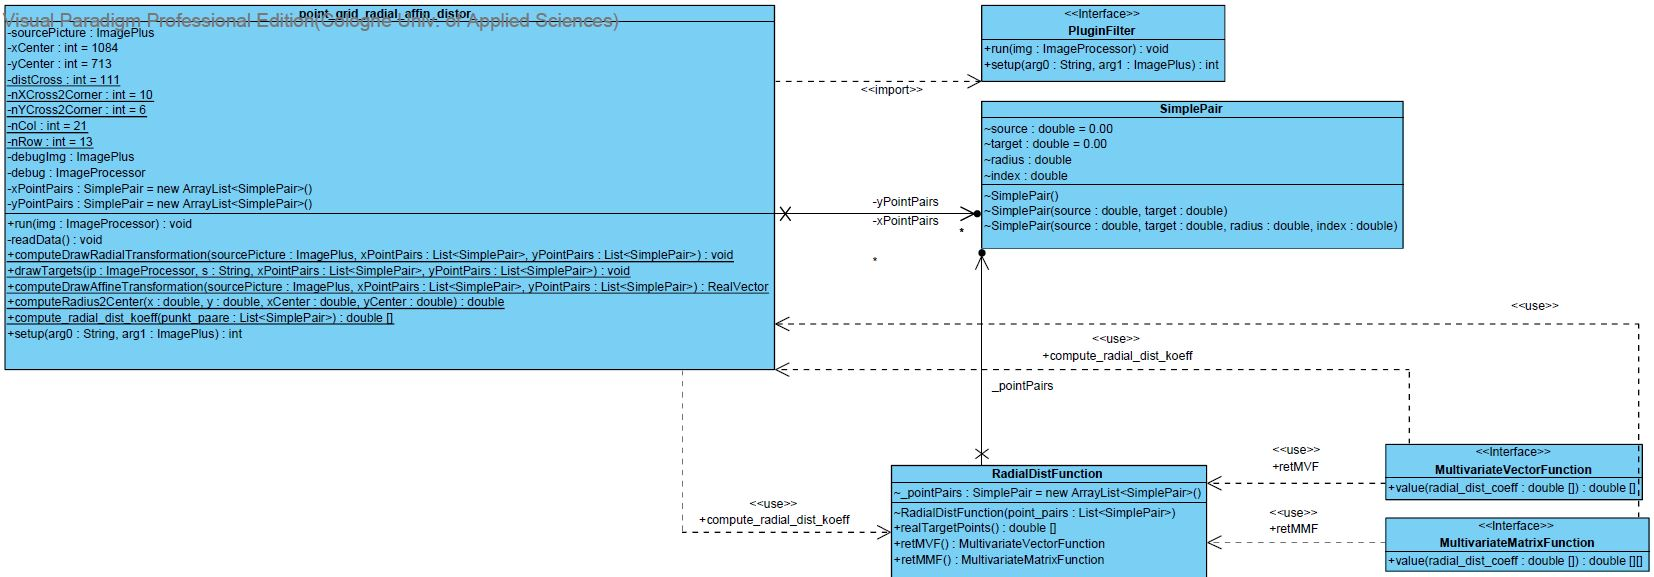
\includegraphics[height=\textheight]{Images/UML.JPG}
\caption{UML Klassendiagramm}
\label{img:UML}
\end{figure}

\newpage
